\section{Асимптотика}

%------------------------------------------------

\begin{frame}
    \center \Huge Асимптотика
\end{frame}

%------------------------------------------------

\begin{frame}
    \frametitle{Логарифм}

    \big 
    $x=\log_a{b}$ это такое число x, что x^a=b

    $4=\log_4{16}$

\end{frame}

%------------------------------------------------

\begin{frame}
    \frametitle{Определение}
    \quad $g(x) = O(f(x)) => \exists C = const : \exists x_1:  \forall x\geq x_1 \Rightarrow Cg(x) \geq f(x)$ 

    \quad Функция $g(x)$ является асимптотической оценкой функции $f(x)$ тогда, когда существует константа $С$, при которой найдётся такой $x_1$, что для любого $x$, не меньшего $x_1$, выполняется неравенство $Cg(x) \geq f(x)$

\end{frame}

%------------------------------------------------

\begin{frame}
    \frametitle{Определение}

    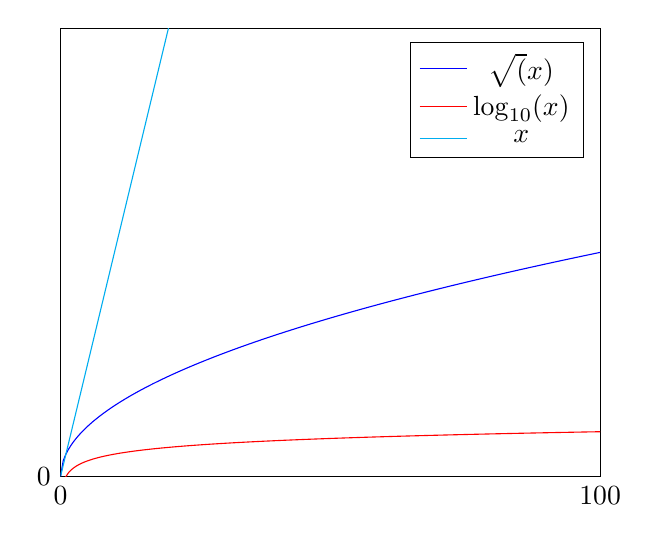
\begin{tikzpicture}
        \begin{axis}[
            xmin=0, xmax=100,
            ymin=0, ymax=20,
            xtick={0,100},
            ytick={0,120},
            legend pos=north east,
            ]

            \addplot[
                color=blue,
                mark=none,
                samples=200,
                domain=0:100,
                unbounded coords=jump
                ]
                {sqrt(x)};

            \addplot[
                color=red,
                mark=none,
                samples=200,
                domain=0:100,
                unbounded coords=jump
                ]
                {log10(x)};

            \addplot[
                color=cyan,
                mark=none,
                samples=200,
                domain=0:100,
                unbounded coords=jump
                ]
                {x};

            \legend{$\sqrt(x)$, 
                    $\log_{10}(x)$,
                    $x$}
        \end{axis}
    \end{tikzpicture}
    \begin{tikzpicture}
        \begin{axis}[
            xmin=0, xmax=1000,
            ymin=-50, ymax=50,
            xtick={1000},
            ytick={0},
            legend pos=south west,
            fr
            ]

            \addplot[
                color=blue,
                mark=none,
                samples=200,
                domain=0:1000,
                unbounded coords=jump
                ]
                {25*sin(x)};

            \addplot[
                color=red,
                mark=none,
                samples=200,
                domain=0:1000,
                unbounded coords=jump
                ]
                {sqrt(x)};

            \addplot[
                color=black,
                mark=none,
                samples=200,
                domain=0:1000,
                unbounded coords=jump
                ]
                {0};

            \legend{$\sin(x)$, 
                    $\sqrt(x)$}
        \end{axis}
    \end{tikzpicture}

\end{frame}

%------------------------------------------------

\begin{frame}
    \frametitle{Частые асимптотики}

    \begin{center}
        \begin{tabular}{|c|c|} 
            \hline
            Асимптотика & Возможный размер данных \\
            \hline
            $a^n$ & примерно никогда \\  
            \hline
            $n!$ & 10 \\  
            \hline
            $n^3$ & 500 \\  
            \hline
            $n^2$ & 10000 \\  
            \hline
            $nlog(n)$ & 10^6 \\  
            \hline
            $n$ & 10^8 \\  
            \hline
            $\sqrt{n}$ & не хватит памяти \\  
            \hline
            $\log{n}$ & не хватит памяти \\  
            \hline
            $1$ & ваще жесть \\  
            \hline
        \end{tabular}
    \end{center}
\end{frame}

%------------------------------------------------

\begin{frame}
    \frametitle{Как считать?}

    \begin{enumerate}
        \item Заведём функцию сложности алгоритма
        \item Посчитаем примерное количество операций
        \item Держим в уме накладные расходы
        \item Придумываем худший случай
    \end{enumerate}
\end{frame}

%------------------------------------------------

\begin{frame}
    \frametitle{Свойства}

    \quad $g(x) = O(f(x)) => \exists C = const : \exists x_1:  \forall x\geq x_1 \Rightarrow Cg(x) \geq f(x)$ 

    \begin{enumerate}
        \item $a=const \Rightarrow O(af(x))=OO(f(x))$
        \item $O(n^2+n+8)=O(n^2)$\\
    \end{enumerate}

     \quad Важно помнить что на самом деле и константы и малые функции всё ещё влияют на временную сложность и могут привести к неверное оценке алгоритма 
\end{frame}

%------------------------------------------------

\begin{frame}
    \frametitle{Почему нет основания логарифма?}
    \quad $O(\log_a{n})=O(\dfrac{\log_b{n}}{\log_b{a}})=\dfrac{1}{\log_b{a}}\log_b{n}\\ \dfrac{1}{\log_b{a}}=const \Rightarrow O(\dfrac{1}{\log_b{a}}\log_b{n})=O(\log_b(n))\Rightarrow O(\log_a{n}) = O(\log_b(n))$

\\
    \quadОпять же, стоит понимать что от основания на самом деле влияет скорость выполнения и для точной оценки его следует писать
\end{frame}

%------------------------------------------------

\begin{frame}[fragile]
    \frametitle{Упражнения}
    
    Сортировка пузырьком
    \begin{cpp}
        for (int i = 0; i < arr.size(); i++) {
            for (int j = 0; j < arr.size()-1; j++) {
                if (arr[j] > arr[j + 1]) {
                    int tmp = arr[j];
                    arr[j] = arr[j + 1];
                    arr[j + 1] = b;
                }
            }
        }
    \end{cpp}
    
\end{frame}

%------------------------------------------------

\begin{frame}[fragile]
    \frametitle{Упражнения}
    
    Сортировка пузырьком
    \begin{cpp}
        for (int i = 0; i < arr.size(); i++) {
            for (int j = 0; j < arr.size()-1; j++) {
                if (arr[j] > arr[j + 1]) {
                    int tmp = arr[j];
                    arr[j] = arr[j + 1];
                    arr[j + 1] = b;
                }
            }
        }
    \end{cpp}

    Ответ: $O(n^2)$

\end{frame}

%------------------------------------------------

\begin{frame}[fragile]
    \frametitle{Упражнения}
    
    \begin{cpp}
        int recursion(n){
            if(n < 1){
                return 1;
            }

            int ans = 0;
            for(int i = 0; i < n){
                ans += recursion(n);
            }

            return ans;
        }
    \end{cpp}
    
\end{frame}

%------------------------------------------------

\begin{frame}[fragile]
    \frametitle{Упражнения}
    
    \begin{cpp}
        int recursion(int n){
            if(n < 1){
                return 1;
            }

            int ans = 0;
            for(int i = 0; i < n){
                ans += recursion(n);
            }

            return ans;
        }
    \end{cpp}
    
    Ответ: $O(n^n)$
\end{frame}

%------------------------------------------------

\begin{frame}[fragile]
    \frametitle{Упражнения}
    
    Дерево Фенвика
    \begin{cpp}
        int sum (int r){
            int result = 0;
            for (int i = r; i >= 0; r = (i & (i+1)) - 1){
                result += t[r];
            }
            return result;
        }
    \end{cpp}
    
\end{frame}

%------------------------------------------------

\begin{frame}[fragile]
    \frametitle{Упражнения}
    
    Дерево Фенвика
    \begin{cpp}
        int sum (int r){
            int result = 0;
            for (int i = r; i >= 0; r = (i & (i+1)) - 1){
                result += t[r];
            }
            return result;
        }
    \end{cpp}
    
    Ответ: $O(log{n})$
\end{frame}

%------------------------------------------------

\begin{frame}[fragile]
    \frametitle{Упражнения}
    
    Дерево Отрезков
    \begin{cpp}
        int sum (int v, int tl, int tr, int l, int r) {
            if (l > r){
                return 0;
            }
            if (l == tl && r == tr){
                return t[v];
            }
            int tm = (tl + tr) / 2;
            return sum (v*2, tl, tm, l, min(r,tm))
            + sum (v*2+1, tm+1, tr, max(l,tm+1), r);
        }
    \end{cpp}
    
\end{frame}

%------------------------------------------------

\begin{frame}[fragile]
    \frametitle{Упражнения}

    Дерево Отрезков
    \begin{cpp}
        int sum (int v, int tl, int tr, int l, int r) {
            if (l > r){
                return 0;
            }
            if (l == tl && r == tr){
                return t[v];
            }
            int tm = (tl + tr) / 2;
            return sum (v*2, tl, tm, l, min(r,tm))
            + sum (v*2+1, tm+1, tr, max(l,tm+1), r);
        }
    \end{cpp}
    
    Ответ: $O(log{n})$
\end{frame}

%------------------------------------------------

\begin{frame}
    \center\huge{Ссылка на тест в телеграме}
    \center
\includegraphics[scale=0.15]{QRtest.png}
\end{frame}

%------------------------------------------------
